% Copyright 2004 by Till Tantau <tantau@users.sourceforge.net>.
%
% In principle, this file can be redistributed and/or modified under
% the terms of the GNU Public License, version 2.
%
% However, this file is supposed to be a template to be modified
% for your own needs. For this reason, if you use this file as a
% template and not specifically distribute it as part of a another
% package/program, I grant the extra permission to freely copy and
% modify this file as you see fit and even to delete this copyright
% notice. 

\documentclass{beamer}
% There are many different themes available for Beamer. A comprehensive
% list with examples is given here:
% http://deic.uab.es/~iblanes/beamer_gallery/index_by_theme.html
% You can uncomment the themes below if you would like to use a different
% one:
%\usetheme{AnnArbor}
%\usetheme{Antibes}
%\usetheme{Bergen}
%\usetheme{Berkeley}
%\usetheme{Berlin}
%\usetheme{Boadilla}
%\usetheme{boxes}
%\usetheme{CambridgeUS}
%\usetheme{Copenhagen}
%\usetheme{Darmstadt}
\usetheme{default}
%\usetheme{Frankfurt}
%\usetheme{Goettingen}
%\usetheme{Hannover}
%\usetheme{Ilmenau}
%\usetheme{JuanLesPins}
%\usetheme{Luebeck}
%\usetheme{Madrid}
%\usetheme{Malmoe}
%\usetheme{Marburg}
%\usetheme{Montpellier}
%\usetheme{PaloAlto}
%\usetheme{Pittsburgh}
%\usetheme{Rochester}
%\usetheme{Singapore}
%\usetheme{Szeged}
%\usetheme{Warsaw}

\usepackage{graphicx}

\title{Presentation Title}

% A subtitle is optional and this may be deleted
\subtitle{Optional Subtitle}

\author{Michi RAKOTONARIVO}
% - Give the names in the same order as the appear in the paper.
% - Use the \inst{?} command only if the authors have different
%   affiliation.

\institute[Universities of Somewhere and Elsewhere] % (optional, but mostly needed)
{
  LJK EDP
}
\date{End Feb  -  end Mars 2018}


\AtBeginSubsection[]
{
  \begin{frame}<beamer>{Outline}
    \tableofcontents[currentsection,currentsubsection]
  \end{frame}
}

% Let's get started
\begin{document}

\begin{frame}{Erreurs Exact/Elements finis}
Pour $N=1000, k=[0,2\pi], E_6$
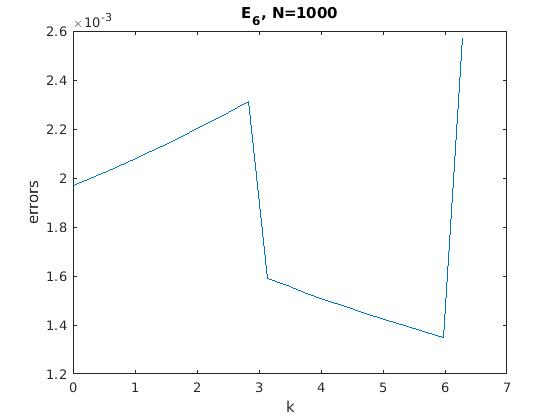
\includegraphics[width=6cm]{ERR_6_rel.jpg} 
 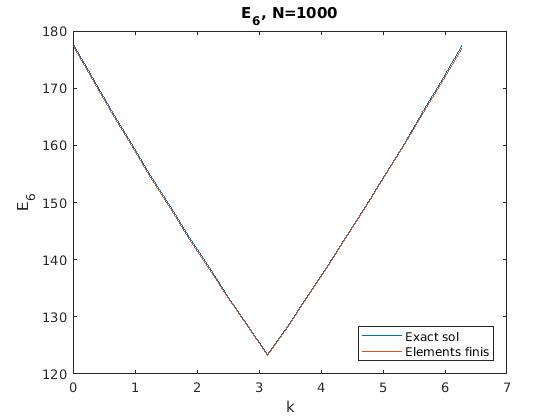
\includegraphics[width=6cm]{ERR_6_comp.jpg} 
\end{frame}



\begin{frame}{Erreurs Exact/Elements finis}
Pour $N=1000, k=[0,2\pi], E_5$
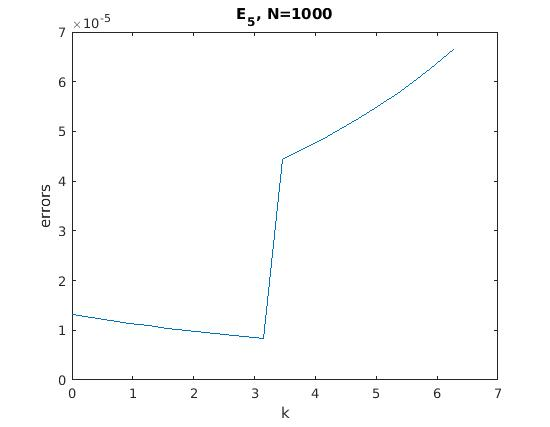
\includegraphics[width=6cm]{ERR_5_rel.jpg} 
 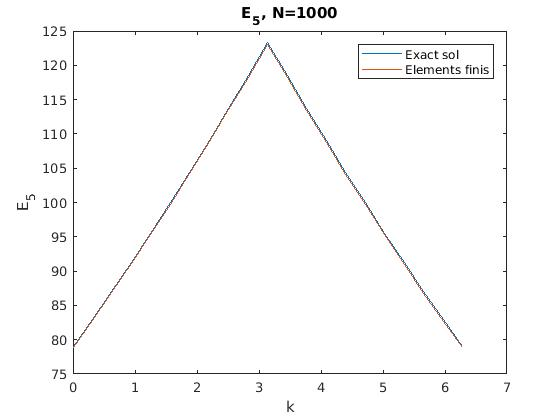
\includegraphics[width=6cm]{ERR_5_comp.jpg} 
\end{frame}

\begin{frame}{Erreurs Exact/Elements finis}
Pour $N=1000, k=[0,2\pi], E_1$
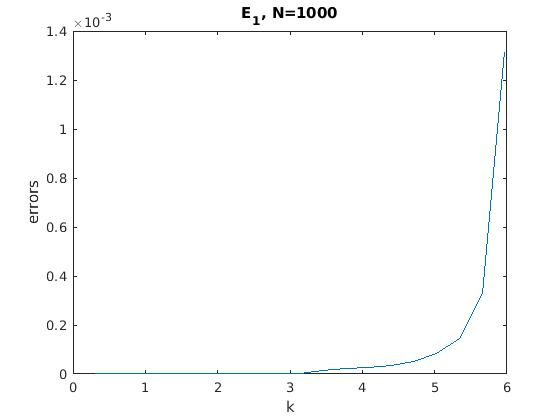
\includegraphics[width=6cm]{ERR_1_rel.jpg} 
 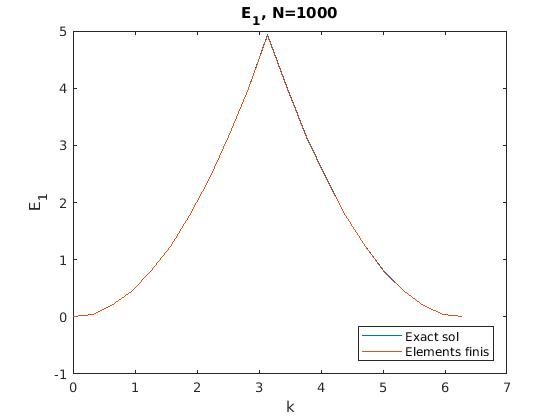
\includegraphics[width=6cm]{ERR_1_comp.jpg} 
\end{frame}

\begin{frame}{Erreurs Exact/Elements/Difference finis}
Pour $dx=[ \frac{1}{1000}, \frac{1}{100}], k=[0,2\pi], E_1(left), E_6(right)$
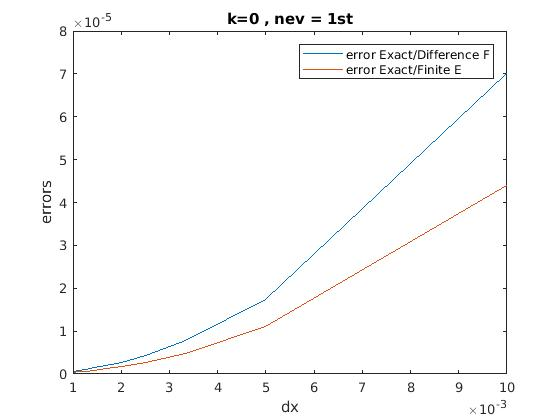
\includegraphics[width=6cm]{ERR_1_k.jpg} 
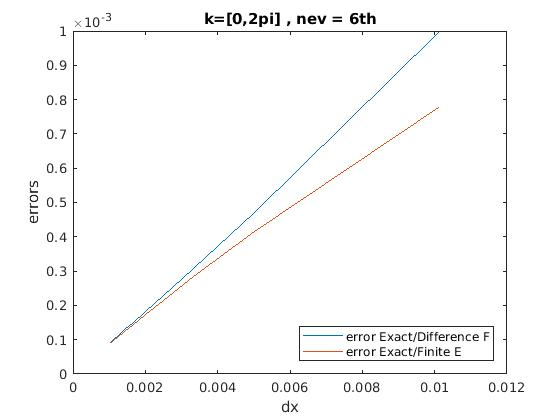
\includegraphics[width=6cm]{ERR_6_k.jpg} 
\end{frame}

\begin{frame}{Erreurs Exact/Elements/Difference finis}
Pour $dx=[ \frac{1}{1000}, \frac{1}{100}], k=[0,2\pi], E_1(left), E_6(right)$
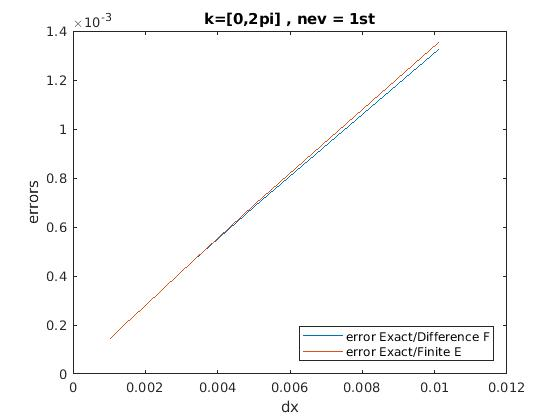
\includegraphics[width=6cm]{ERR_1_k_bis.jpg} 
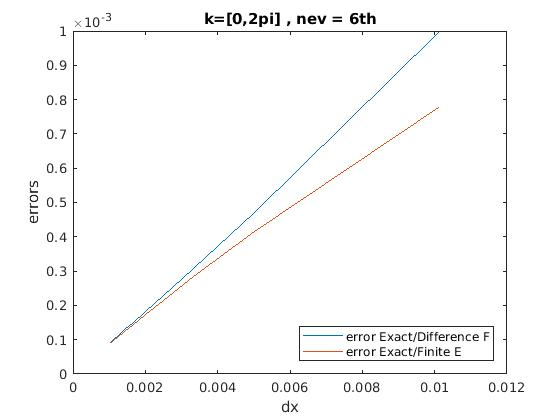
\includegraphics[width=6cm]{ERR_6_k.jpg} 
\end{frame}

\end{document}







